\documentclass[10pt]{article}

% ============================================================
% PACKAGES
% ============================================================

\usepackage{amsmath}
\usepackage{amssymb}
\usepackage{comment}
\usepackage{fancyhdr}
\usepackage{hyperref}
\usepackage{listings}
\usepackage{longdivision}
\usepackage{booktabs}
\usepackage{polynom}
\usepackage{graphicx}
\usepackage{tikz}
\usepackage{float}
\usepackage{cancel}
\usepackage{xlop}
\usepackage{xcolor}

\graphicspath{{figures/}}

% Creative Commons license
\usepackage{ccicons}
\usepackage[
    type={CC},
    modifier={by-nc-sa},
    version={4.0},
]{doclicense}


% ============================================================
% GENERAL FORMATTING
% ============================================================

\setlength{\parindent}{0pt}
\setlength{\parskip}{0.5em}


% ============================================================
% HYPERREF
% ============================================================

\hypersetup{
    colorlinks=true,
    linkcolor=blue,
    urlcolor=blue,
    citecolor=blue
}


% ============================================================
% PAGE STYLE
% ============================================================

\pagestyle{fancy}

\fancyhf{}

\fancyfoot[C]{%
    \small\textcolor{gray}{%
        GitHub repository:
        \href{https://github.com/deepak-venkatesh/gelfand-geometry}
        {github.com/deepak-venkatesh/gelfand-geometry}
    }%
}

\fancyfoot[R]{\thepage}

\renewcommand{\headrulewidth}{0pt}
\renewcommand{\footrulewidth}{0.4pt}


% ============================================================
% TITLE
% ============================================================

\title{%
    An Unofficial Compendium of Worked Solutions to the Problems in
    \textit{Geometry}\\[0.5em]
    \large
    by I.\,M.~Gelfand \& T.~Alekseyevskaya (Gelfand)
}

\author{Deepak Venkatesh}

\date{\today}


% ============================================================
% CUSTOM STRUCTURE FOR GELFAND'S GEOMETRY
% ============================================================

% Major Parts I--IV
\newcounter{geompart}

% Chapter counter
\newcounter{geomchapter}

% Problem counter
\newcounter{problem}

% Appendix subsection counter
\newcounter{appendixsection}


% ============================================================
% MAJOR PART
%
% Calling \geompart resets:
%
%   chapter -> 0
%   problem -> 0
%
% Therefore the first chapter/problem becomes 1.
% ============================================================

\newcommand{\geompart}[1]{%

    \clearpage

    \stepcounter{geompart}

    \setcounter{geomchapter}{0}
    \setcounter{problem}{0}

    \phantomsection

    \addcontentsline
        {toc}
        {part}
        {Part \Roman{geompart}: #1}

    \begin{center}

        \vspace*{3em}

        {\Huge\bfseries
        Part \Roman{geompart}}

        \vspace{1.5em}

        \begin{minipage}{0.82\textwidth}
            \centering
            \Large\bfseries
            #1
        \end{minipage}

        \vspace{3em}

    \end{center}

    \clearpage
}


% ============================================================
% SUBPART
%
% Used only in Parts II and IV.
%
% IMPORTANT:
%
% This does NOT reset chapters.
% This does NOT reset problems.
%
% Example:
%
% \geomsubpart{I}{Lines and Segments}
% ============================================================

\newcommand{\geomsubpart}[2]{%

    \clearpage

    \phantomsection

    \addcontentsline
        {toc}
        {section}
        {Part #1: #2}

    \begin{center}

        \vspace*{1em}

        {\Large\bfseries
        Part #1}

        \vspace{0.5em}

        {\LARGE\bfseries
        #2}

        \vspace{1.5em}

    \end{center}
}


% ============================================================
% CHAPTER
%
% Problems do NOT reset when a new chapter begins.
%
% Example:
%
% \geomchapter{Points and lines}
% ============================================================

\newcommand{\geomchapter}[1]{%

    \clearpage

    \stepcounter{geomchapter}

    \phantomsection

    \addcontentsline
        {toc}
        {subsection}
        {Chapter \arabic{geomchapter}: #1}

    {\Large\bfseries
    Chapter \arabic{geomchapter}. #1}

    \vspace{1em}
}


% ============================================================
% PROBLEM ENVIRONMENT
%
% Example:
%
% \begin{problem}
%
% Solution goes here.
%
% \end{problem}
%
%
% Optional text:
%
% \begin{problem}[Additional note]
%
% ...
%
% \end{problem}
% ============================================================

\newenvironment{problem}[1][]{%

    \refstepcounter{problem}

    \par
    \medskip

    \noindent
    \textbf{%
        Problem~\arabic{problem}.%
        \if\relax\detokenize{#1}\relax
        \else
            \ #1%
        \fi
    }

    \par
    \vspace{0.5em}

}{%

    \par
    \vspace{1em}

}


% ============================================================
% APPENDIX FOR CHAPTER II
%
% This resets ONLY the problem counter.
%
% Thus:
%
%   Part II main problems:       Problem 1--59
%   Appendix for Chapter II:     Problem 1--16
%
% It does NOT alter the main chapter counter.
% ============================================================

\newcommand{\chapterappendix}[1]{%

    \clearpage

    \setcounter{problem}{0}
    \setcounter{appendixsection}{0}

    \phantomsection

    \addcontentsline
        {toc}
        {section}
        {Appendix for Chapter #1}

    \begin{center}

        {\LARGE\bfseries
        Appendix for Chapter #1}

    \end{center}

    \vspace{1.5em}
}


% ============================================================
% APPENDIX SECTION
%
% The Appendix for Chapter II itself contains five named
% sections. These are separate from the main chapter counter.
%
% Example:
%
% \appendixsection{Why we cannot define equal segments...}
% ============================================================

\newcommand{\appendixsection}[1]{%

    \stepcounter{appendixsection}

    \phantomsection

    \addcontentsline
        {toc}
        {subsection}
        {\arabic{appendixsection}. #1}

    \vspace{1em}

    {\large\bfseries
    \arabic{appendixsection}. #1}

    \vspace{0.75em}
}


% ============================================================
% DOCUMENT
% ============================================================

\begin{document}


% ============================================================
% TITLE
% ============================================================

\maketitle


% ============================================================
% ABSTRACT
% ============================================================

\begin{abstract}

\noindent This book is an independent and unofficial collection of worked solutions
to problems inspired by the book \textit{Geometry} by
I.\,M.~Gelfand and T.~Alekseyevskaya (Gelfand), first published in 2020.\\

\noindent The original text presents a wide range of problems in projective geometry,
affine geometry, symplectic geometry, and Euclidean geometry. The book
contains solved exercises and questions, but the reader is also given over
200 problems to solve.\\

\noindent The aim of this book is to provide clear, logically consistent solutions
to all unsolved problems addressed, written in a style accessible to
motivated students and self-learners.\\

\noindent Figures are either drawn by hand and scanned, constructed using GeoGebra,
or produced directly in \LaTeX. Where applicable, proofs or calculations
may also be checked using computer programs written in Scheme
(a dialect of Lisp) or Python.\\

\noindent Large language models were used only as auxiliary tools, primarily for
generating figures in \LaTeX\ and for reviewing exposition.\\

\noindent This work is not affiliated with, endorsed by, or approved by the original
authors or publisher. Any errors, omissions, or inconsistencies are
entirely my own.\\

\noindent Issues and corrections may be reported at the
\href{https://github.com/deepak-venkatesh/gelfand-geometry/issues}
{project repository}.

\end{abstract}


% ============================================================
% COPYRIGHT AND DISCLAIMER
% ============================================================

\clearpage

\thispagestyle{empty}

\vspace*{2cm}

\begin{center}

    {\Large\textbf{Copyright and Disclaimer}}

\end{center}

\vspace{1cm}


\textbf{Unofficial companion.}

\vspace{0.4cm}

This document is an
\textbf{independent, unofficial collection of worked solutions}
to problems from \textit{Geometry} by
I.\,M.~Gelfand and T.~Alekseyevskaya (Gelfand)
(first published in 2020).

\vspace{0.4cm}

This work is
\textbf{not affiliated with, endorsed by, or approved by}
the original authors or the publisher. The names of the authors
and the title of the book are used only for identification and
reference.

\vspace{0.4cm}

The original problem statements are not reproduced here.
All exposition and solutions are written independently by the
author of this document.

\vspace{1.5cm}

\textbf{Copyright \textcopyright\ \the\year\ Deepak Venkatesh}

\vspace{1.5cm}

License:

\doclicenseThis

\vfill

Project repository:

\href{https://github.com/deepak-venkatesh/gelfand-geometry}
{https://github.com/deepak-venkatesh/gelfand-geometry}


% ============================================================
% OPTIONAL LICENSE PAGE
% ============================================================

\begin{comment}

\clearpage

\vspace*{27em}

\doclicenseThis

\end{comment}


% ============================================================
% DEDICATION
% ============================================================

\clearpage

\thispagestyle{empty}

\vspace*{\fill}

\begin{center}

    \textit{For}\\[0.5em]

    \textit{My Daughter and Son}

\end{center}

\vspace*{\fill}


% ============================================================
% TABLE OF CONTENTS
% ============================================================

\clearpage

\tableofcontents


% ============================================================
% WORKING NOTES
% ============================================================

\clearpage

\section*{Working Notes}

\addcontentsline{toc}{section}{Working Notes}


\textit{Challenging Problems for Middle Schoolers:}


\vspace{1em}


\textit{Typographical Errors:}

\begin{enumerate}
    \item The standard mathematical spelling of Hermann Minkowski's name is \textit{Minkowski} and not \textit{Minkowsky}.
\end{enumerate}



% ============================================================
% INTRODUCTION
%
% This is NOT part of the numbered chapters.
% ============================================================

\clearpage

\section*{Introduction}

\addcontentsline{toc}{section}{Introduction}

No problems in this chapter.


%%%%%%%%%%%%%%%%%%%%%%%%%%%%%%%%%%%%%%%%%%%%
%                                          %
%           END OF CHAPTER                 %
%                                          %
%%%%%%%%%%%%%%%%%%%%%%%%%%%%%%%%%%%%%%%%%%%



% ############################################################
%
% PART I
%
% POINTS AND LINES:
% A LOOK AT PROJECTIVE GEOMETRY
%
% Chapters 1--14
% Problems 1--53
%
% ############################################################

\geompart{Points and Lines: A Look at Projective Geometry}



% ============================================================
% PART I --- CHAPTER 1
% ============================================================

\geomchapter{Points and lines}

% Insert problems here.

% Example:
%
% \begin{problem}
%
% Your solution.
%
% \end{problem}

\begin{problem}
In a line if we place a point we divide it into 2 parts. In this case both the part are \emph{rays} and the point is an \emph{endpoint}.

Now if there are 2 point on the line, we still have 2 rays but the two endpoints create a line segment. 

So $n$ points on a line will give 2 rays and $(n - 1)$ line segments.

For this problem.

\[
\begin{array}{lcl}
  n = 100\\
  \text{endpoints} = 100\\
  \text{rays} = 2\\
  \text{segments} = 100 - 1 = 99
\end{array}
\]

\begin{center}
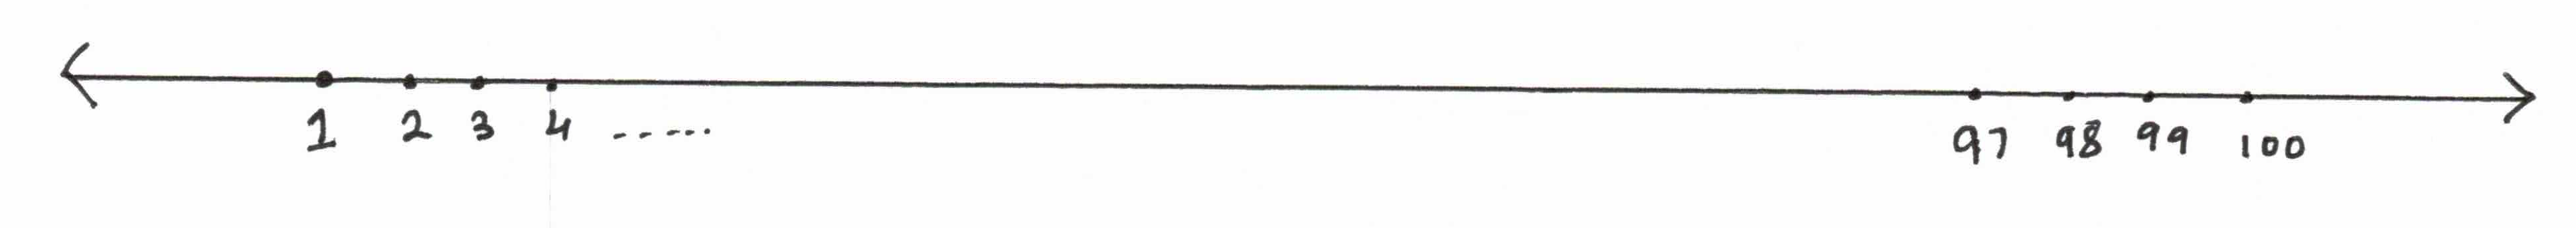
\includegraphics[width=1\textwidth]{p1-c01-prob01.png}  
\end{center}

\end{problem}

\begin{problem}

Three possibilities exist:\\
1. The two lines $A$ and $B$ can perfectly coincide.\\
2. They can be parallel to each other.\\
3. They can intersect at some point.\\

Basis the figure below the plane can be divided into 2, 3, or 4 parts.

\begin{center}
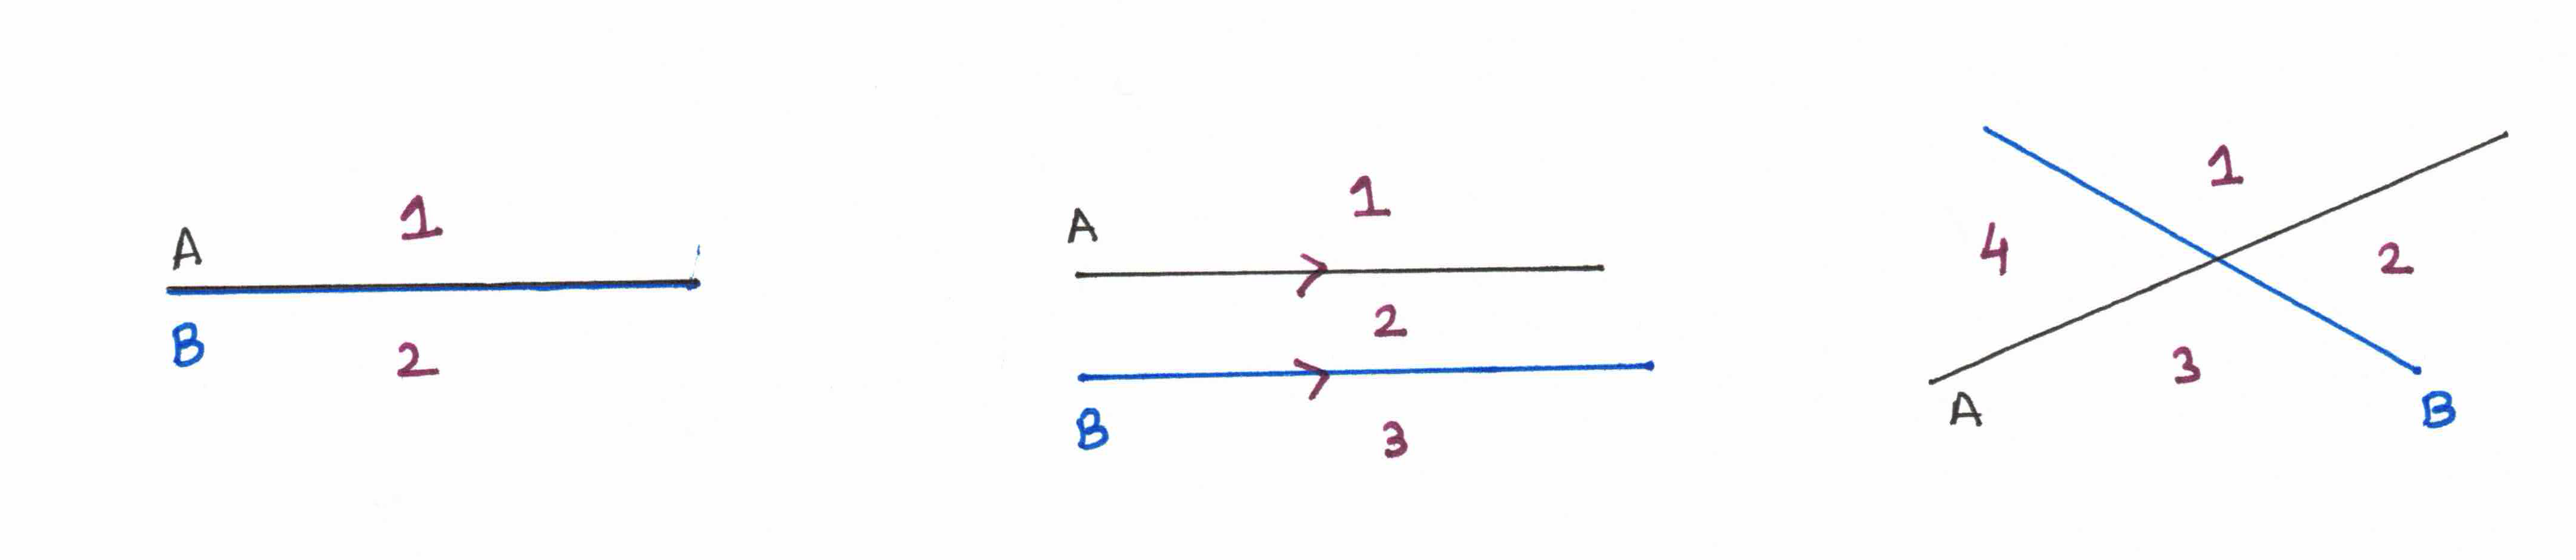
\includegraphics[width=1\textwidth]{p1-c01-prob02.png}  
\end{center}
\end{problem}

\begin{problem}
The chapter explains that geometric constructions performed using the two axioms below are call constructions in \emph{projective geometry}.\\

\textbf{Axiom 1}: Through any two points, one can draw a unique line.\\

\textbf{Axiom 2}: Any two lines either have a unique point of intersection or do not intersect (are parallel).\\

Basis these two axioms of projective geometry we can construct the line $AC$.

\begin{center}
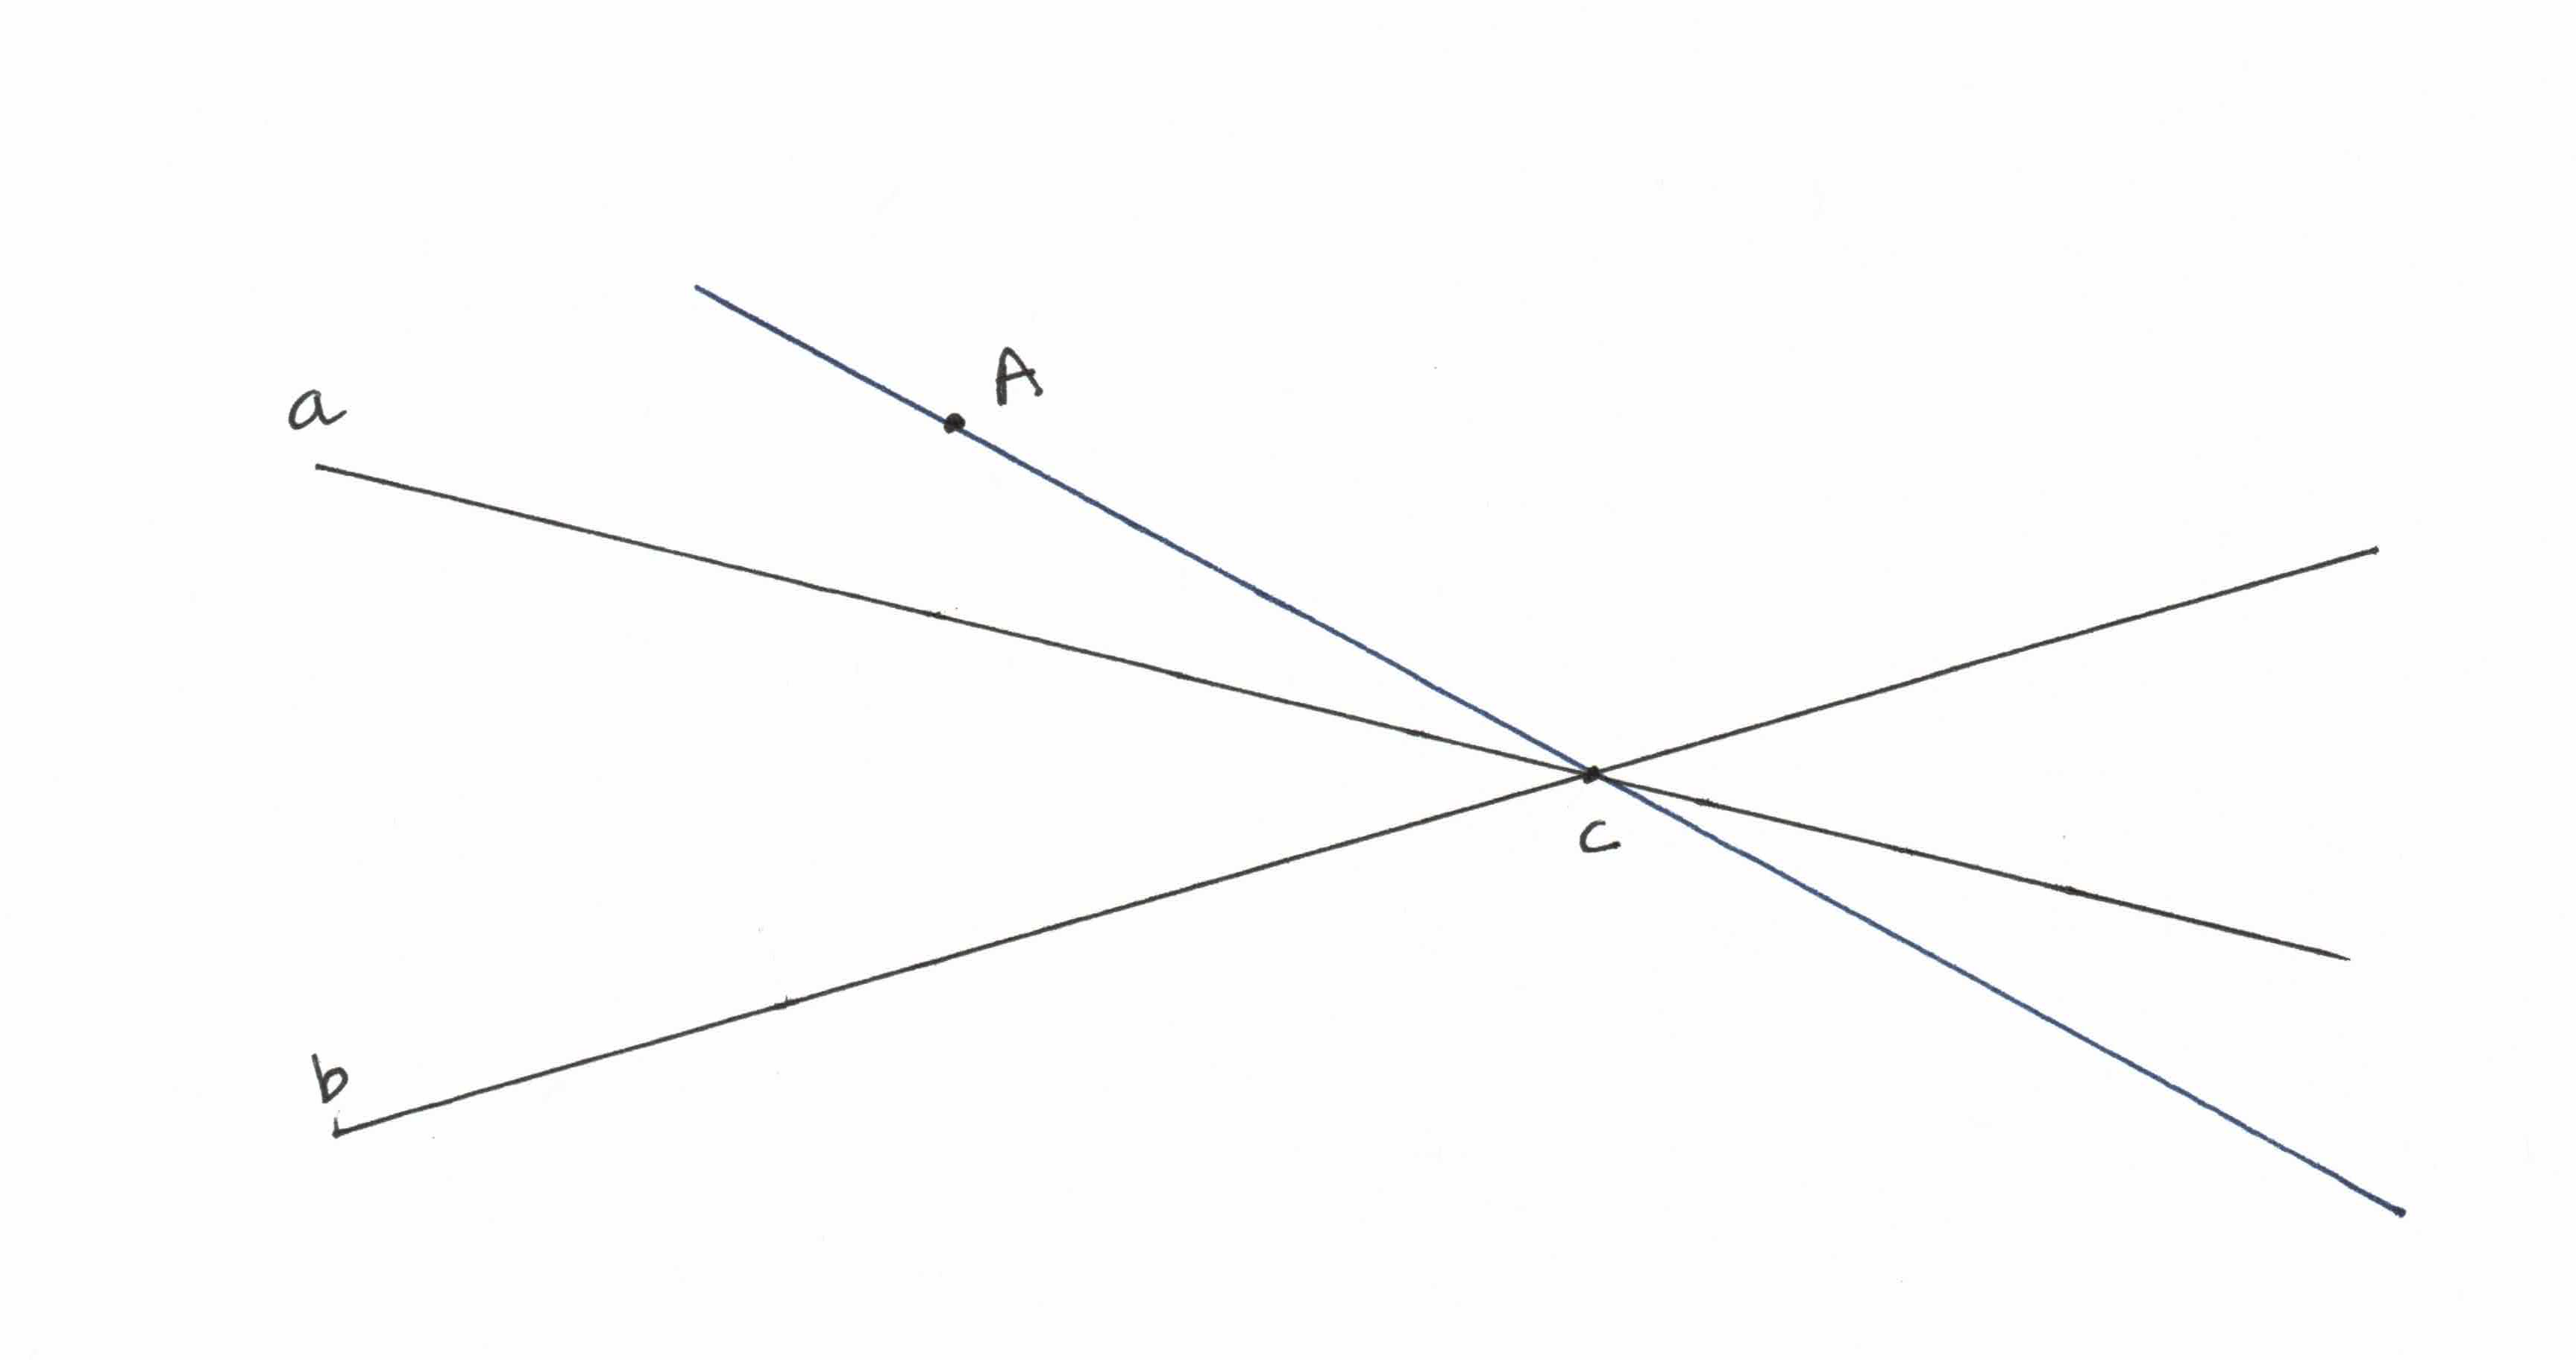
\includegraphics[width=1\textwidth]{p1-c01-prob03.png}  
\end{center}
\end{problem}

% ============================================================
% PART I --- CHAPTER 2
% ============================================================

\geomchapter{Two lines and an angle}

% Insert problems here.



% ============================================================
% PART I --- CHAPTER 3
% ============================================================

\geomchapter{Three lines}

% Insert problems here.



% ============================================================
% PART I --- CHAPTER 4
% ============================================================

\geomchapter{Four lines. Quadrilaterals}

% Insert problems here.



% ============================================================
% PART I --- CHAPTER 5
% ============================================================

\geomchapter{Five lines}

% Insert problems here.



% ============================================================
% PART I --- CHAPTER 6
% ============================================================

\geomchapter{Projection from a point onto a line}

% Insert problems here.



% ============================================================
% PART I --- CHAPTER 7
% ============================================================

\geomchapter{Dual configurations in projective geometry}

% Insert problems here.



% ============================================================
% PART I --- CHAPTER 8
% ============================================================

\geomchapter{Desargues configuration}

% Insert problems here.



% ============================================================
% PART I --- CHAPTER 9
% ============================================================

\geomchapter{Dual Desargues configuration}

% Insert problems here.



% ============================================================
% PART I --- CHAPTER 10
% ============================================================

\geomchapter{Algebraic notation of ``computer presentation'' of configurations}

% Insert problems here.



% ============================================================
% PART I --- CHAPTER 11
% ============================================================

\geomchapter{Polygons and $n$ straight lines}

% Insert problems here.



% ============================================================
% PART I --- CHAPTER 12
% ============================================================

\geomchapter{Convex polygons, convex hull of $n$ points}

% Insert problems here.



% ============================================================
% PART I --- CHAPTER 13
% ============================================================

\geomchapter{Solution of Exercise 3 with the help of a Desargues configuration}

% Insert problems here.



% ============================================================
% PART I --- CHAPTER 14
% ============================================================

\geomchapter{Overview of Chapter I}

% Insert problems here.



% ############################################################
%
% PART II
%
% PARALLEL LINES:
% A LOOK AT AFFINE GEOMETRY
%
% Main chapters 1--13
% Main problems 1--59
%
% Three subparts
%
% Appendix for Chapter II:
% Problems restart at 1
%
% ############################################################

\geompart{Parallel Lines: A Look at Affine Geometry}



% ============================================================
%
% PART II --- SUBPART I
%
% LINES AND SEGMENTS
%
% ============================================================

\geomsubpart{I}{Lines and Segments}



% ============================================================
% PART II --- CHAPTER 1
% ============================================================

\geomchapter{Parallel Straight Lines}

% Insert problems here.



% ============================================================
% PART II --- CHAPTER 2
% ============================================================

\geomchapter{Operations available in Chapter II}

% Insert problems here.



% ============================================================
% PART II --- CHAPTER 3
% ============================================================

\geomchapter{Properties of parallel lines}

% Insert problems here.



% ============================================================
% PART II --- CHAPTER 4
% ============================================================

\geomchapter{Segments lying on parallel lines}

% Insert problems here.



% ============================================================
%
% PART II --- SUBPART II
%
% FIGURES
%
% Chapter numbering continues.
% Problem numbering continues.
%
% ============================================================

\geomsubpart{II}{Figures}



% ============================================================
% PART II --- CHAPTER 5
% ============================================================

\geomchapter{Parallelograms}

% Insert problems here.



% ============================================================
% PART II --- CHAPTER 6
% ============================================================

\geomchapter{Triangles}

% Insert problems here.



% ============================================================
% PART II --- CHAPTER 7
% ============================================================

\geomchapter{Trapezoids}

% Insert problems here.



% ============================================================
%
% PART II --- SUBPART III
%
% OPERATIONS WITH FIGURES
%
% ============================================================

\geomsubpart{III}{Operations with Figures}



% ============================================================
% PART II --- CHAPTER 8
% ============================================================

\geomchapter{The Minkowsky addition of two figures}

% Insert problems here.



% ============================================================
% PART II --- CHAPTER 9
% ============================================================

\geomchapter{Parallel projection}

% Insert problems here.



% ============================================================
% PART II --- CHAPTER 10
% ============================================================

\geomchapter{Parallel translation}

% Insert problems here.



% ============================================================
% PART II --- CHAPTER 11
% ============================================================

\geomchapter{Central symmetry on the plane}

% Insert problems here.



% ============================================================
% PART II --- CHAPTER 12
% ============================================================

\geomchapter{Vectors}

% Insert problems here.



% ============================================================
% PART II --- CHAPTER 13
% ============================================================

\geomchapter{Overview of Chapter II}

% Insert problems here.



% ============================================================
%
% APPENDIX FOR CHAPTER II
%
% Problem numbering restarts here.
%
% Appendix Problem 1
% ...
% Appendix Problem 16
%
% ============================================================

\chapterappendix{II}



% ------------------------------------------------------------
% Appendix Section 1
% ------------------------------------------------------------

\appendixsection{Why we cannot define equal segments in Chapter II}

% Insert appendix problems here.
%
% The FIRST problem inserted here automatically becomes
% Problem 1.



% ------------------------------------------------------------
% Appendix Section 2
% ------------------------------------------------------------

\appendixsection{Parallel lines, equal segments, and the Desargues configuration}

% Problem numbering continues.



% ------------------------------------------------------------
% Appendix Section 3
% ------------------------------------------------------------

\appendixsection{Arithmetic operations with segments}

% Problem numbering continues.



% ------------------------------------------------------------
% Appendix Section 4
% ------------------------------------------------------------

\appendixsection{Segments and rational numbers}

% Problem numbering continues.



% ------------------------------------------------------------
% Appendix Section 5
% ------------------------------------------------------------

\appendixsection{Affine coordinate systems on the plane}

% Problem numbering continues through Problem 16.



% ############################################################
%
% PART III
%
% AREA:
% A LOOK AT SYMPLECTIC GEOMETRY
%
% Chapters 1--8
% Problems 1--27
%
% ############################################################

\geompart{Area: A Look at Symplectic Geometry}



% ============================================================
% PART III --- CHAPTER 1
% ============================================================

\geomchapter{The area of a figure}

% Insert problems here.



% ============================================================
% PART III --- CHAPTER 2
% ============================================================

\geomchapter{Area of a parallelogram}

% Insert problems here.



% ============================================================
% PART III --- CHAPTER 3
% ============================================================

\geomchapter{Area of a triangle}

% Insert problems here.



% ============================================================
% PART III --- CHAPTER 4
% ============================================================

\geomchapter{Area of a trapezoid}

% Insert problems here.



% ============================================================
% PART III --- CHAPTER 5
% ============================================================

\geomchapter{Area of a polygon}

% Insert problems here.



% ============================================================
% PART III --- CHAPTER 6
% ============================================================

\geomchapter{More problems on areas}

% Insert problems here.



% ============================================================
% PART III --- CHAPTER 7
% ============================================================

\geomchapter{How to measure the area of a figure}

% Insert problems here.



% ============================================================
% PART III --- CHAPTER 8
% ============================================================

\geomchapter{Overview of Chapter III}

% Insert problems here.



% ############################################################
%
% PART IV
%
% CIRCLES:
% A LOOK AT EUCLIDEAN GEOMETRY
%
% Chapters 1--24
% Problems 1--75
%
% Three subparts
%
% ############################################################

\geompart{Circles: A Look at Euclidean Geometry}



% ============================================================
%
% PART IV --- SUBPART I
%
% INTRODUCTION TO THE CIRCLE
%
% ============================================================

\geomsubpart{I}{Introduction to the Circle}



% ============================================================
% PART IV --- CHAPTER 1
% ============================================================

\geomchapter{Operations available in Chapter IV}

% Insert problems here.



% ============================================================
% PART IV --- CHAPTER 2
% ============================================================

\geomchapter{Comparing segments}

% Insert problems here.



% ============================================================
% PART IV --- CHAPTER 3
% ============================================================

\geomchapter{Angles}

% Insert problems here.



% ============================================================
% PART IV --- CHAPTER 4
% ============================================================

\geomchapter{Operations with figures}

% Insert problems here.



% ============================================================
%
% PART IV --- SUBPART II
%
% THE GEOMETRY OF THE TRIANGLE AND OTHER FIGURES
%
% Chapters and problems continue without resetting.
%
% ============================================================

\geomsubpart{II}{The Geometry of the Triangle and Other Figures}



% ============================================================
% PART IV --- CHAPTER 5
% ============================================================

\geomchapter{Elements of triangle. Congruent triangles}

% Insert problems here.



% ============================================================
% PART IV --- CHAPTER 6
% ============================================================

\geomchapter{Construction of a triangle from its elements}

% Insert problems here.



% ============================================================
% PART IV --- CHAPTER 7
% ============================================================

\geomchapter{Relations between elements of a triangle}

% Insert problems here.



% ============================================================
% PART IV --- CHAPTER 8
% ============================================================

\geomchapter{Properties of a triangle. Particular kinds of triangles}

% Insert problems here.



% ============================================================
% PART IV --- CHAPTER 9
% ============================================================

\geomchapter{Area in Euclidean geometry}

% Insert problems here.



% ============================================================
% PART IV --- CHAPTER 10
% ============================================================

\geomchapter{The Pythagorean theorem and its applications}

% Insert problems here.



% ============================================================
% PART IV --- CHAPTER 11
% ============================================================

\geomchapter{Relations between lines and points}

% Insert problems here.



% ============================================================
% PART IV --- CHAPTER 12
% ============================================================

\geomchapter{Special lines and special points in a triangle}

% Insert problems here.



% ============================================================
% PART IV --- CHAPTER 13
% ============================================================

\geomchapter{Polygons}

% Insert problems here.



% ============================================================
% PART IV --- CHAPTER 14
% ============================================================

\geomchapter{Summary of facts about different quadrilaterals}

% Insert problems here.



% ============================================================
% PART IV --- CHAPTER 15
% ============================================================

\geomchapter{Similarity}

% Insert problems here.



% ============================================================
%
% PART IV --- SUBPART III
%
% CIRCLES
%
% Chapters continue from 16.
% Problems continue without resetting.
%
% ============================================================

\geomsubpart{III}{Circles}



% ============================================================
% PART IV --- CHAPTER 16
% ============================================================

\geomchapter{Circles and points}

% Insert problems here.



% ============================================================
% PART IV --- CHAPTER 17
% ============================================================

\geomchapter{Circles and lines}

% Insert problems here.



% ============================================================
% PART IV --- CHAPTER 18
% ============================================================

\geomchapter{Two or more circles}

% Insert problems here.



% ============================================================
% PART IV --- CHAPTER 19
% ============================================================

\geomchapter{Circles and angles}

% Insert problems here.



% ============================================================
% PART IV --- CHAPTER 20
% ============================================================

\geomchapter{A circle and a triangle}

% Insert problems here.



% ============================================================
% PART IV --- CHAPTER 21
% ============================================================

\geomchapter{Circles and polygons}

% Insert problems here.



% ============================================================
% PART IV --- CHAPTER 22
% ============================================================

\geomchapter{Circumference and arc}

% Insert problems here.



% ============================================================
% PART IV --- CHAPTER 23
% ============================================================

\geomchapter{Disks and sectors}

% Insert problems here.



% ============================================================
% PART IV --- CHAPTER 24
% ============================================================

\geomchapter{Overview of Chapter IV}

% Insert problems here.



% ============================================================
% END DOCUMENT
% ============================================================

\end{document}